\documentclass[table]{manual}
\setjobnamebeamerversion{main.beamer} 

\pagestyle{fancy}
\rhead{\LaTeX}
\lhead{\LaTeX\ in 30 Minuten}
\rfoot{\thepage}

\title{Modul 150}
\subtitle{E-Business-Applikationen anpassen}

\date{\today}
\author{abc}
\author{\href{mailto:daniel.senften@talent-factory.ch}{Daniel Senften}}


% ----------------------------------

\begin{document}

    % TODO In der endgültigen Version des Dokumentes den Befehl auskommentieren
    \fxsetup{draft}

    \setmainfont{Verdana}
    \DeclareGraphicsExtensions{.pdf,.jpg,.tif}
    \maketitle
    \pagestyle{fancy}
    \newpage
    
    \tableofcontents % Inhaltsverzeichnis
    \listoffixmes

    \parindent0em\parskip1em
    \newpage

    \mode*

\setmonofont{Verdana}

% ===========================================================================
\begin{frame}[fragile]
    \frametitle<presentation>{Was ist \LaTeX?}

    \begin{itemize}
        \item \LaTeX\ ist ein Werkzeug zur Erstellung professionell aussehender Dokumente.
        \item Es basiert auf der WYSIWYM-Idee (\emph{what you see is what you mean}),
        d.h.~Sie konzentrieren sich nur auf den Inhalt Ihres Dokuments und der Computer
        kümmert sich um die Formatierung.
        \item Anstatt wie bei Microsoft Word oder LibreOffice Text auf einer Seite zur
        Steuerung der Formatierung zu einzufügen, können Benutzer reinen Text
        eingeben und \LaTeX\ den Rest überlassen.
    \end{itemize}
\end{frame}

% ===========================================================================
\begin{frame}[fragile]
    \frametitle<presentation>{Warum sollte ich \LaTeX\ nutzen?}

    \begin{itemize}
        \item\LaTeX\ wird weltweit für wissenschaftliche Dokumente, Bücher und
        viele andere Formen der Veröffentlichung eingesetzt.
        \item Es kann nicht nur wunderschöne Dokumente erstellen, sondern
        ermöglicht es den Benutzern auch, sehr schnell die komplexeren Teile
        des Satzes anzugehen, wie z.B.~die Eingabe von Mathematik, die Erstellung
        von Inhaltsverzeichnissen, die Referenzierung und Erstellung von
        Bibliographien,$\ldots$
        \item Einer der wichtigsten Gründe, warum man \LaTeX\ verwendet, ist,
        dass es den Inhalt des Dokuments vom Stil trennt.
    \end{itemize}

\end{frame}


% ===========================================================================
\begin{frame}[fragile]
    \frametitle<presentation>{Standardabweichung}

    \begin{center}

        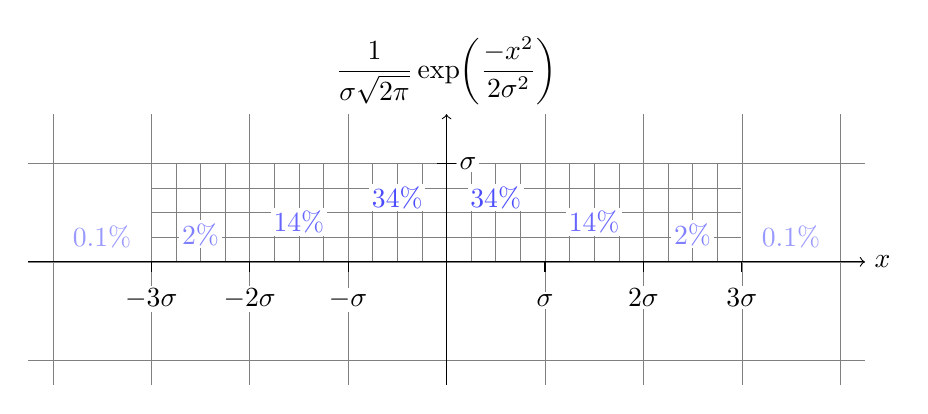
\begin{tikzpicture}[scale=1.25]
            \colorlet{col1}{blue!70}
            \colorlet{col2}{blue!60}
            \colorlet{col3}{blue!50}
            \colorlet{col4}{blue!40}
            \draw [help lines] (-4.25,-1.25) grid (4.25,1.5);
            \draw [help lines,step=0.25cm] (-2.99,0) grid (2.99,0.99);

            \draw[->] (0,-1.25) -- (0,1.5) node [above]
            {$\displaystyle
            \frac{1}{\sigma\sqrt{2\pi}}\exp\biggl(\frac{-x^2}{2\sigma^2}\biggr)
            $};

            \begin{scope}[smooth,draw=gray!20,y=0.3989422804cm]
                \filldraw [fill=col3] plot[id=f1,domain=-3:-2] function {exp(-x*x/2)}
                -- (-2,0) -- (-3,0) -- cycle;
                \filldraw [fill=col2] plot[id=f2,domain=-2:-1] function {exp(-x*x/2)}
                -- (-1,0) -- (-2,0) -- cycle;
                \filldraw [fill=col1] plot[id=f3,domain=-1:0]  function {exp(-x*x/2)}
                -- (0,0)  -- (-1,0) -- cycle;
                \filldraw [fill=col1] plot[id=f4,domain=0:1] function {exp(-x*x/2)}
                -- (1,0)  --  (0,0) -- cycle;
                \filldraw [fill=col2] plot[id=f5,domain=1:2] function {exp(-x*x/2)}
                -- (2,0)  -- (1,0) -- cycle;
                \filldraw [fill=col3] plot[id=f6,domain=2:3] function {exp(-x*x/2)}
                -- (3,0)  -- (2,0) -- cycle;
                \draw[black] plot[id=f7,domain=-4.25:4.25,samples=100]
                function {exp(-x*x/2)};
            \end{scope}
            \draw[->] (-4.25,0) -- (4.25,0) node [right] {$x$};

            \foreach \pos/\label in {-3/$-3\sigma$,-2/$-2\sigma$,-1/$-\sigma$,
            1/$\sigma$,2/$2\sigma$,3/$3\sigma$}
            \draw (\pos,0) -- (\pos,-0.1) (\pos cm,-3ex) node
            [anchor=base,fill=white,inner sep=1pt]  {\label};

            \draw (-0.1,1) -- (.1,1) node [right,fill=white,inner sep=1pt] {$\sigma$};

            \foreach \pos/\percent/\height in {1/34/0.5,2/14/0.25,3/2/0.125,4/0.1/0.1}
            {
            \node[text=col\pos,anchor=base,yshift=2pt,xshift=-0.625cm,
            fill=white,inner sep=1pt] at (\pos,\height) {$\percent\%$};
            \node[text=col\pos,anchor=base,yshift=2pt,xshift=.625cm,
            fill=white,inner sep=1pt]  at (-\pos,\height) {$\percent\%$};
            }
        \end{tikzpicture}
    \end{center}

\end{frame}

% ===========================================================================
\begin{frame}[fragile]
    \frametitle<presentation>{Einfache Funktionen}
    \begin{center}
        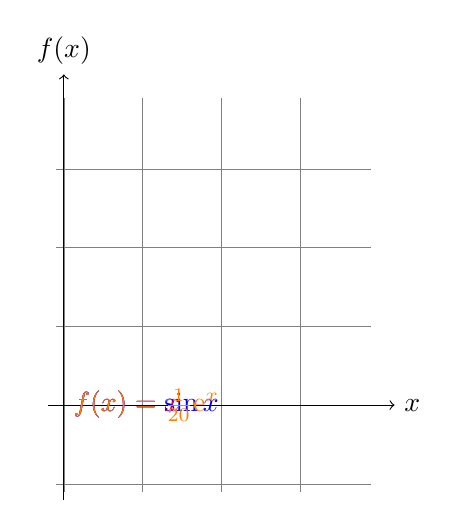
\begin{tikzpicture}[domain=0:4]
            \draw[very thin,color=gray] (-0.1,-1.1) grid (3.9,3.9);
            \draw[->] (-0.2,0) -- (4.2,0) node[right] {$x$};
            \draw[->] (0,-1.2) -- (0,4.2) node[above] {$f(x)$};
            \draw[color=red] plot[id=x] function{x}
            node[right] {$f(x) =x$};
            \draw[color=blue] plot[id=sin] function{sin(x)}
            node[right] {$f(x) = \sin x$};
            \draw[color=orange] plot[id=exp] function{0.05*exp(x)}
            node[right] {$f(x) = \frac{1}{20} \mathrm e^x$};
        \end{tikzpicture}
    \end{center}
\end{frame}


% ===========================================================================
\begin{frame}[fragile]
    \frametitle<presentation>{Mein erstes \LaTeX\ Dokument}
    \inputminted[frame=single]{latex}{examples/first.tex}
\end{frame}


% ===========================================================================
\begin{frame}[fragile]
    \frametitle<presentation>{Die Präambel eines Dokuments}

    \begin{minted}[frame=single,autogobble]{latex}
        \documentclass[12pt, letterpaper]{article}
        \RequirePackage[utf8]{inputenc}
    \end{minted}
\end{frame}


% ===========================================================================
\begin{frame}[fragile]
    \frametitle<presentation>{Titel, Autor, Datum,$\ldots$}

    \begin{minted}[frame=single,autogobble]{latex}
        \documentclass[12pt, a4, twoside]{manual}
        \RequirePackage[german]{babel}
        \selectlanguage{german}

        \title{Mein erstes Dokument}
        \author{Daniel Senften
        \thanks{unterstützt durch das Talent Factory Team}}
        \date{\today}

        % Weiterer Text...
    \end{minted}
\end{frame}


% ===========================================================================
\begin{frame}[fragile]
\frametitle<presentation>{Fett, kursiv und unterstrichen}

    \begin{itemize}
        \item \textbf{Fettgedruckter} gedruckter Text wird in \LaTeX\ mit dem Befehl
            \mintinline{latex}{\textbf{...}} geschrieben.
        \item \textit{Kursivschrift} kann mit \mintinline{latex}{\textit{...}}
            erreicht werden.
        \item Für \underline{unterstrichenen} Text steht
            \mintinline{latex}{\underline{...}} zur Verfügung.
    \end{itemize}

\end{frame}


% ===========================================================================
\begin{frame}[fragile]
    \frametitle<presentation>{Hinzufügen von Bildern}
    \inputminted[frame=single]{latex}{examples/images.tex}
\end{frame}



%    \newpage\appendix
%    \section{Verzeichnisse}
%    \parindent0em\parskip0em
%    \listoffigures   % Abbildungsverzeichnis
%    \listoftables    % Tabellenverzeichnis
%    \listofexercises % Liste der Übungen
%
%    \renewcommand{\listoflistingscaption}{Programmbeispiele}
%    \listoflistings
%
%    \bibliographystyle{plain} % We choose the "plain" | "alpha" reference style
%    \bibliography{bibliography}

\end{document}
